\documentclass{article}
\usepackage{graphicx} % Required for inserting images
\usepackage{times}
\usepackage{fancyhdr} % Required for header and footer
\usepackage{algorithm} % Required for algorithm environment
\usepackage{algpseudocode} % Required for algorithmic environment
\usepackage{tikz}
\usetikzlibrary{matrix}
\usepackage{subcaption}

\pagestyle{fancy}
\fancyhf{} % Clear default header/footer
\lhead{\small Department of Computer Science}
\rhead{\small University of Massachusetts, Amherst}

\title{\Large Monte Carlo Tree Search (MCTS), REINFORCE with baseline and Actor Critic}
\author{
  \begin{tabular}{cc}
    \small Avinash Nandyala & \small Sneha Sree Vavilapalli \\
    \small Department of Computer Science & \small Department of Computer Science \\
    \small University of Massachusetts, Amherst & \small University of Massachusetts, Amherst \\
    \small anandyala@umass.edu & \small svavilapalli@umass.edu
  \end{tabular}
}
\date{}
\begin{document}

\maketitle
\thispagestyle{fancy}

\section{Introduction}

In this project, we have implemented three influential algorithmic approaches in reinforcement learning: a) Monte Carlo Tree Search (MCTS), b) REINFORCE with baseline, and c) Actor-Critic methods. 
Each algorithm represents different paradigms in solving sequential decision-making problems.

Monte Carlo Tree Search (MCTS) stands out as a powerful decision-time planning algorithm that has revolutionized artificial intelligence, particularly in game-playing domains. 
Most notably, MCTS was instrumental in advancing computer Go from amateur level in 2005 to grandmaster level by 2015, forming the foundation for AlphaGo's historic achievements.
MCTS combines tree search with Monte Carlo sampling, making it particularly effective in domains with large state spaces.

REINFORCE with baseline, a policy gradient method, represents a different approach to reinforcement learning. 
By incorporating a baseline function, it addresses the high variance issues common in basic policy gradient methods. 
This algorithm learns both a policy and a value function, with the latter serving to reduce variance in gradient estimates while maintaining unbiased updates.

Actor-Critic methods bridge the gap between value-based and policy-based approaches. 
By maintaining separate networks for policy (actor) and value function (critic), these methods combine the advantages of both paradigms. 
The critic's value estimates help reduce variance in the actor's policy updates while maintaining the ability to learn stochastic policies.

We evaluated these algorithms across three distinct environments:
\begin{itemize}
    \item The 687-gridworld environment, a classic grid-based navigation task with stochastic transitions and obstacles
    \item The Acrobot environment, a challenging control problem requiring precise joint manipulation
    \item The Cat Vs Monsters environment, a modified grid world featuring dynamic obstacles and multiple threat types
    \item Cliff walking environment, grid-based task with deterministic transitions and presence of cliff which penalizes the reward that needs to be avoided. When training the initial state is chosen to be from a set of valid possible states because when it is fixed to (3,0) it was computationally inefficient.
\end{itemize}

In the following sections, we provide detailed descriptions of each environment and algorithm, followed by comprehensive experimental results and comparative analyses. Our evaluations focus on learning efficiency, convergence properties, and final performance across these diverse environments. Through this study, we aim to understand the strengths and limitations of each approach in different types of reinforcement learning problems.

\section{Environments}

\subsection{687-gridworld}

This is a grid world environment with a 5x5 grid. The agent has 4 actions: up, down, left, and right.
The agent starts at the top left corner and the goal is to reach the bottom right corner.
The agent has to avoid obstacles and water.
For transitioning, the agent has an 80 percent chance to perform the intended action, a 5 percent chance to malfunction and move right, a 5 percent chance to move left, and a 10 percent chance to stay in place.
The agent gets a reward of -10 if it reaches water, 10 if it reaches the goal, and 0 for each step taken.
The first state is $S_0 = (0,0)$ and the goal state is $S_{\infty} = (4,4)$. Obstacles are at $(2,2)$ and $(3,2)$. Water is at $(4,2)$.

\subsection{Cat Vs Monsters}

This is a grid world environment with a 5x5 grid.
The cat agent starts at the top left corner and the goal is to reach the bottom right corner.
The cat agent has to avoid the furniture and the monsters. For transitioning, the agent has a 70 percent chance to perform the intended action, a 12 percent chance to malfunction and move right, a 12 percent chance to move left, and an 8 percent chance to stay in place.
The cat agent gets a reward of -8 if it reaches monsters, 10 if it reaches the goal, and -0.05 for each step taken.
The first state is $S_0 = (0,0)$ and the goal state is $S_{\infty} = (4,4)$.
Furniture is at $(2,1)$, $(2,2)$, $(2,3)$, $(3,2)$. Monsters are at $(4,2)$, $(0,3)$.

\subsection{Acrobot}

This is a classic control environment consisting of two links connected linearly to form a chain, with one end fixed.
The agent controls the joint between the two links by applying torque (-1, 0, or 1).
The goal is to swing the free end of the chain above a given height while starting from a hanging downward position.
For each state, the agent observes 6 values: cosine and sine of both joint angles ie., $\theta_1$ and $\theta_2$, and their angular velocities ie., $\omega_1$ and $\omega_2$.
The agent receives a reward of -1 for each step and 0 when reaching the goal height. And reward threshold is -100
The episode terminates when either the goal height is reached which can be calculated mathematically by $-cos(\theta_1)-cos(\theta_1+\theta_2)>1.0$ or it terminates after 500 steps.
The starting state is uniformy distributed by $cos(\theta_1), sin(\theta_1), cos(\theta_2), sin(\theta_2), \omega_1, \omega_2 \in [-0.1,0.1]$.
Constraints are $\theta_1, \theta_2 \in [-\pi, \pi]$ rads, $\omega_1 \in [-4\pi, 4\pi]$ rads/sec, $\omega_2 \in [-9\pi, 9\pi]$ rads/sec.

\subsection{Cliff Walking}
This is an (4 * 12) grid based env where the agent starts at a given state (3,0) and its goal is to reach the goal state on the other side of the cliff which is (3,12). The states in between (3, 0) and (3, 12) is completely cliff. The agent can choose one of the four actions possible which is from (Up, Down, Left, Right). There is no stochastic transition probability associated, but deterministic, which implies all actions taken are implemented with a probability of 1. The agent receives a reward of -1 for each step taken and -100 when it enters the cliff. The episode ends when we reach the terminal goal state or when number of steps exceed 1000. $\gamma$ chosen here is 0.9. 




\section{Algorithms}

\subsection{Monte Carlo Tree Search (MCTS)}

Monte Carlo Tree Search (MCTS) is a decision-time planning algorithm that combines tree search with Monte Carlo sampling to evaluate actions. 
It builds a search tree incrementally by running simulations, focusing computational resources on the most promising lines of play. 
The algorithm is particularly effective in domains with large state spaces where traditional search methods are impractical.

It has 4 main steps:
\begin{itemize}
    \item \textbf{Selection:} Begin at the root node and navigate the tree using the Upper Confidence bounds for Trees (UCT) algorithm:
    \item \textbf{Expansion:} Add one or more child nodes to the selected node and move to that node
    \item \textbf{Simulation:} From the new node, simulate to a terminal state or maximum depth which is a hyperparameter using a random rollout policy.
    \item \textbf{Backpropagation:} Update statistics (visits and values of all nodes)
\end{itemize}
\begin{figure}
    \centering
    \includegraphics[width=1\linewidth]{3.1.png}
    \caption{MCTS Flow}
    \label{fig:3.1}
\end{figure}
\begin{algorithm}
\caption{Monte Carlo Tree Search}
\begin{algorithmic}[1]
\State Initialize root node with current state
\While{computational budget remains}
    \State \textbf{Selection:}
    \State \hspace{\algorithmicindent} Starting from root, traverse tree using UCT:
    \State \hspace{\algorithmicindent} $UCT(node) = \frac{wins}{visits} + C\sqrt{\frac{\ln(N)}{visits}}$
    \State \hspace{\algorithmicindent} Until reaching either:
    \State \hspace{\algorithmicindent} - Unexpanded node, or
    \State \hspace{\algorithmicindent} - Terminal state
    \State \textbf{Expansion:}
    \State \hspace{\algorithmicindent} If node not terminal:
    \State \hspace{\algorithmicindent} Add one or more child nodes to tree
    \State \textbf{Simulation:}
    \State \hspace{\algorithmicindent} From new node, simulate to terminal state
    \State \hspace{\algorithmicindent} Using random rollout policy
    \State \textbf{Backpropagation:}
    \State \hspace{\algorithmicindent} Update statistics (visits and values of all nodes)
    \State \hspace{\algorithmicindent} For all nodes traversed in this iteration
\EndWhile
\State \Return action with highest visit count at root
\end{algorithmic}
\label{alg:mcts}
\end{algorithm}

The MCTS algorithm balances exploration and exploitation using the UCT formula, where $C$ is an exploration constant (typically $\sqrt{2}$), $N$ is the parent node's visit count, and $total\_value/visits$ represents the node's average value. 
It has several advantages, including being an anytime algorithm that can return a result at any time with quality improving with more computation, asymmetric tree growth that focuses search on promising moves, requiring no domain-specific knowledge beyond game rules, and being effective in large state spaces where full tree search is impractical. 
MCTS has been particularly successful in game-playing domains, most notably in computer Go, where it formed the basis for AlphaGo's groundbreaking success.



\subsection{REINFORCE with baseline}

REINFORCE with baseline is an extension of the basic REINFORCE algorithm that introduces a baseline function to reduce variance in policy gradient estimates while maintaining unbiased updates.
The baseline function estimates the state value, which is then subtracted from the returns to create an advantage estimate.

The algorithm updates both a policy network $\pi(a|s,\theta)$ and a baseline value function $\hat{v}(s,\mathbf{w})$ using the following steps in the pseudo algorithm below:

\begin{algorithm}
\caption{REINFORCE with Baseline}
\begin{algorithmic}[1]
\State Initialize policy parameters $\theta$ and baseline parameters $\mathbf{w}$
\For{each episode}
    \State Generate trajectory following policy $\pi(a|s,\theta)$
    \For{each timestep $t$ in the episode}
        \State Calculate return $G_t = \sum_{k=t+1}^T \gamma^{k-t-1}R_k$
        \State Calculate advantage estimate $\delta = G_t - \hat{v}(S_t,\mathbf{w})$
        \State Update baseline weights: $\mathbf{w} \leftarrow \mathbf{w} + \alpha^w \delta \nabla \hat{v}(S_t,\mathbf{w})$
        \State Update policy parameters: $\theta \leftarrow \theta + \alpha^\theta \gamma^t \delta \nabla \ln \pi(A_t|S_t,\theta)$
    \EndFor
\EndFor
\end{algorithmic}
\end{algorithm}

The baseline helps reduce variance in the gradient estimates without biasing them, as the baseline is subtracted from the return before computing the policy gradient.
This typically leads to faster and more stable learning compared to the basic REINFORCE algorithm. 
The algorithm uses two learning rates: $\alpha^w$ for the baseline updates and $\alpha^\theta$ for the policy updates.

\subsection{Actor Critic}

Actor-Critic methods combine policy gradient with value function approximation, where the "Actor" learns a policy and the "Critic" learns to evaluate the policy. Unlike REINFORCE with baseline, Actor-Critic methods use the value function to bootstrap the return estimation, making them fully online and incremental. This method is foundational to approaches such as A3C(Asynchronous Advantage Actor-Critic) and PPO (Proximal Policy Optimization) 

The algorithm maintains two networks:
\begin{itemize}
    \item Actor: Policy network $\pi(a|s,\theta)$ that determines action selection
    \item Critic: Value network $\hat{v}(s,\mathbf{w})$ that estimates state values
\end{itemize}

The algorithm updates both a policy network $\pi(a|s,\theta)$ and a baseline value function $\hat{v}(s,\mathbf{w})$ using the following steps in the pseudo algorithm below:

\begin{algorithm}
\caption{Actor-Critic (episodic)}
\begin{algorithmic}[1]
\State Initialize policy parameters $\theta$ and value parameters $\mathbf{w}$
\For{each episode}
    \State Initialize state $S$
    % \State Initialize eligibility traces $\mathbf{z}^\theta = \mathbf{0}$, $\mathbf{z}^w = \mathbf{0}$
    \State $I \leftarrow 1$
    \While{$S$ is not terminal}
        \State Select action $A \sim \pi(\cdot|S,\theta)$
        \State Take action $A$, observe $R$, $S'$
        \State Calculate TD error: $\delta = R + \gamma\hat{v}(S',\mathbf{w}) - \hat{v}(S,\mathbf{w})$
        \State Update critic: $\mathbf{w} \leftarrow \mathbf{w} + \alpha^w \delta \nabla \hat{v}(S,\mathbf{w})$
        \State Update actor: $\theta \leftarrow \theta + \alpha^\theta I \delta \nabla \ln \pi(A|S,\theta)$
        \State $I \leftarrow \gamma I$
        \State $S \leftarrow S'$
\EndFor
\end{algorithmic}
\end{algorithm}

\section{Implementation and Results}


\subsubsection{MCTS}
\textbf{Preliminary Implementation}\\

MCTS has four main hyperparameters: depth and budget. 
Budget $b$ is the number of simulations or time limitation we can have, performed by the MCTS. In our implementation, we have used iterations as the budget. 
Depth Limit $d$ is the depth of the tree which is the maximum depth the MCTS searches with rollout policy.
UCT constant $c$ is the exploration constant which is used to balance exploration and exploitation.
Discount factor $\gamma$ is the discount factor used in the MCTS.\\

We have tested the MCTS on Acrobot, 687-gridworld, cliff walking and cat vs monsters domains. Except for Acrobot, the rest were discrete. 
So, we have tested the MCTS on all the domains with different depths and budgets.
For all the domains, we have taken the average of 5 runs for each depth and budget. \\

\textbf{Observations:}\\
\textbf{Impact of Budget Parameter:}
We can see from the plots (Figures \ref{fig:4.1.1}, \ref{fig:4.2.1}, \ref{fig:4.3.1}, \ref{fig:4.4.1}) that the Average of Estimated Return$(V(S_0))$ from $S_0$ to $S_{\infty}$ is increasing with the budget as it learns better policies.\\

\textbf{Impact of Depth Parameter:}
The impact of depth limit varies across different environments. For the 687-Grid World (Figure \ref{fig:4.1.2}), increasing depth generally leads to improved returns with some variance, as the agent can better plan longer trajectories to reach the goal. 
In contrast, Cliff Walking (Figure \ref{fig:4.2.2}) shows optimal performance up to a depth of 50, after which returns begin to decline, likely due to the increased risk of falling off the cliff with longer planning horizons. 
For Acrobot (Figure \ref{fig:4.3.2}), deeper searches help discover better swing-up strategies, though with diminishing returns at very high depths. The Cat vs Monsters domain (Figure \ref{fig:4.4.2}) benefits from increased depth as it allows the agent to better plan escape routes while avoiding monsters.\\

\textit{Note: Light blue color in the plots represents the range of $V(S_0)$, dark blue line represents the Average of $V(S_0)$ and the shaded area represents the range of returns.}


\begin{figure}[!hb]
    \centering
    \begin{minipage}{0.48\textwidth}
        \centering
        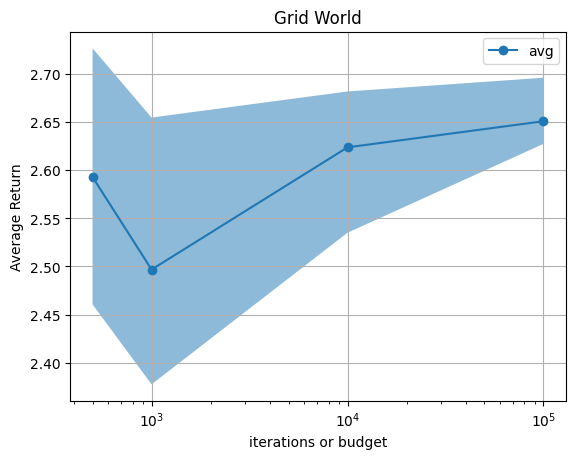
\includegraphics[width=\linewidth]{mcts_grid_budget.png}
        \caption{Average return vs. MCTS budget for 687-Grid World. Each point is the average return from 5 runs. Parameters: UCT with c=2, $\gamma=0.99$, depth=200.}
        \label{fig:4.1.1}
    \end{minipage}
    \hfill
    \begin{minipage}{0.48\textwidth}
        \centering
        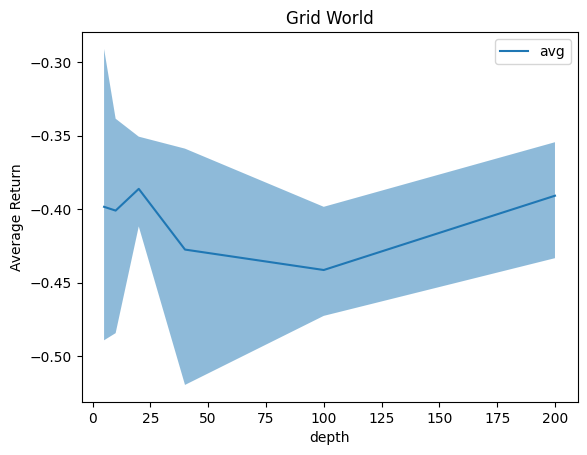
\includegraphics[width=\linewidth]{mcts_grid_depth.png}
        \caption{ Average return vs. MCTS depth for 687-Grid World. Each point is the average return from 5 runs. Parameters: UCT with c=2, $\gamma=0.99$, budget=10000.}
        \label{fig:4.1.2}
    \end{minipage}
\end{figure}
% \textbf{Cliff Walking}
\begin{figure}[!hb]
    \centering
    \begin{minipage}{0.48\textwidth}
        \centering
        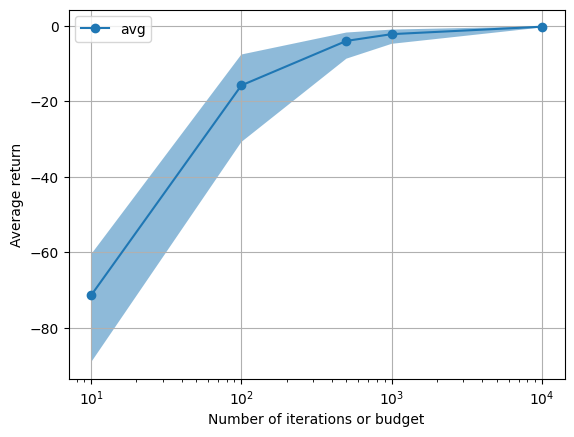
\includegraphics[width=\linewidth]{mcts_cw_budget.png}
        \caption{Average return vs. MCTS budget for Cliff Walking. Each point is the average return from 5 runs. Parameters: UCT with c=5, $\gamma=0.9$, depth=50.}
        \label{fig:4.2.1}
    \end{minipage}
    \hfill
    \begin{minipage}{0.48\textwidth}
        \centering
        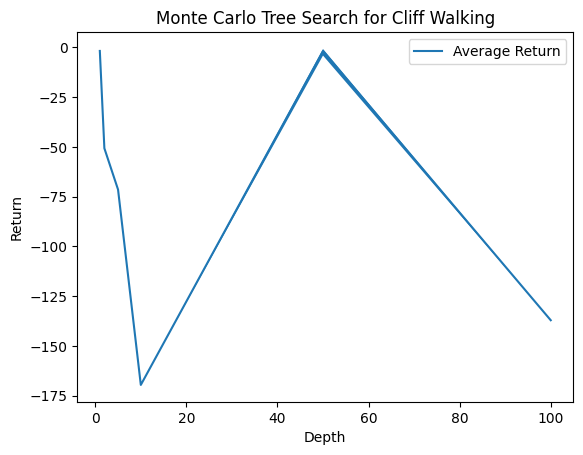
\includegraphics[width=\linewidth]{mcts_cw_depth.png}
        \caption{Average return vs. MCTS depth for Cliff Walking. Each point is the average return from 5 runs. Parameters: UCT with c=5, $\gamma=0.9$, budget=10000.}
        \label{fig:4.2.2}
    \end{minipage}
\end{figure}

\begin{figure}[!hb]
    \centering
    \begin{minipage}{0.48\textwidth}
        \centering
        \includegraphics[width=\linewidth]{mcts_acrobot_budget.png}
        \caption{Average return vs. MCTS budget for Acrobot. Each point is the average return from 5 runs. Parameters: UCT with c=2, $\gamma=1$, depth=100.}
        \label{fig:4.3.1}
    \end{minipage}
    \hfill
    \begin{minipage}{0.48\textwidth}
        \centering
        \includegraphics[width=\linewidth]{mcts_acrobot_depth.png}
        \caption{Average return vs. MCTS depth for Acrobot. Each point is the average return from 5 runs. Parameters: UCT with c=2, $\gamma=1$, budget=500.}
        \label{fig:4.3.2}
    \end{minipage}
\end{figure}

\begin{figure}[!hb]
    \centering
    \begin{minipage}{0.48\textwidth}
        \centering
        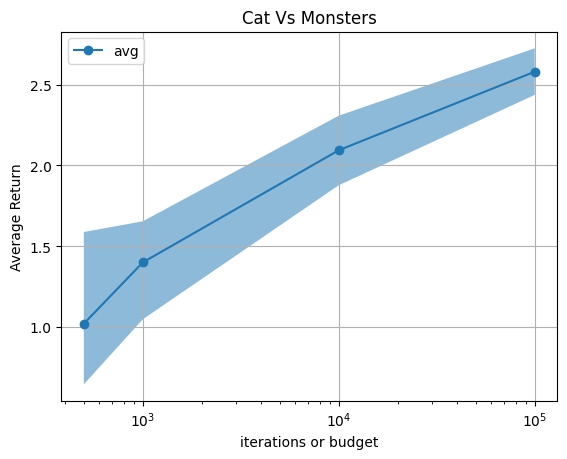
\includegraphics[width=\linewidth]{mcts_cvm_b.png}
        \caption{Average return vs. MCTS budget for Cat vs Monsters. Each point is the average return from 5 runs. Parameters: UCT with c=4, $\gamma=0.925$, depth=200.}
        \label{fig:4.4.1}
    \end{minipage}
    \hfill
    \begin{minipage}{0.48\textwidth}
        \centering
        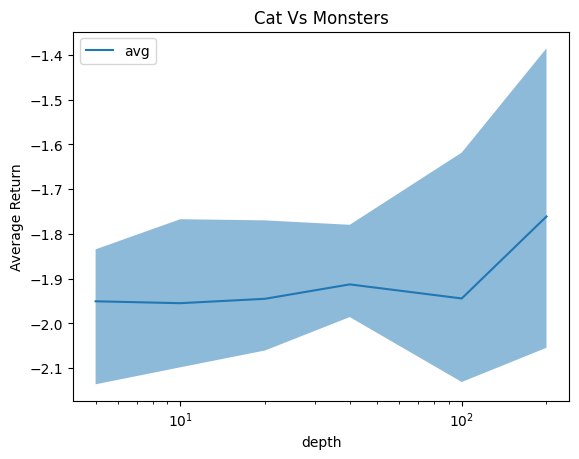
\includegraphics[width=\linewidth]{mcts_cvm_d.png}
        \caption{Average return vs. MCTS depth for Cat vs Monsters. Each point is the average return from 5 runs. Parameters: UCT with c=4, $\gamma=0.925$, budget=10000.}
        \label{fig:4.4.2}
    \end{minipage}
\end{figure}


\textbf{Policy Finding Implementation:}

We know that acrobot is a continuous domain. So, we have used a neural network to approximate the policy and value function.

Other domains are discrete. So, we have used a table to approximate the policy and value function, 
I traversed the entire state space and stored the value function and policy for each state. Here is the psuedocode for the implementation for discrete functions

\begin{algorithm}[H]
\caption{Policy Finding Implementation using MCTS}
\begin{algorithmic}[1]
\State Initialize empty policy table $\pi$ and value table $V$
\State $S \gets$ set of all states in environment
\For{$s \in S$} 
    \State $a, optimalValue \gets$ RunMCTS($s$) \Comment{Get best action from MCTS search}
    \State $\pi[s] \gets a$ \Comment{Store action in policy}
    \State $V[s] \gets optimalValue$\Comment{Store reward in value table} 
\EndFor
\State \Return $\pi, V$ \Comment{Return policy and value function(only for discrete)} 
\end{algorithmic}
\end{algorithm}

If we use the same implementation for continuous domains, we will have to traverse the entire state space which is not feasible.
So, we have used a neural networks to approximate the policy and value function for continuous domains.

for acrobot, we have used a neural network to approximate the policy and value function.
\begin{figure}[H]
    \centering
    \begin{minipage}{0.48\textwidth}
        \centering
        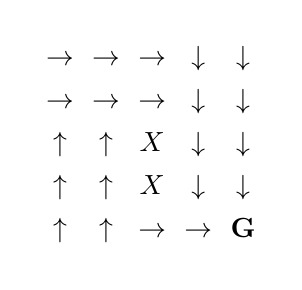
\begin{tikzpicture}
            \matrix (m) [matrix of nodes] {
                $\rightarrow$ & $\rightarrow$ & $\rightarrow$ & $\downarrow$ & $\downarrow$ \\
                $\rightarrow$ & $\rightarrow$ & $\rightarrow$ & $\downarrow$ & $\downarrow$ \\
                $\uparrow$ & $\uparrow$ & $X$ & $\downarrow$ & $\downarrow$ \\
                $\uparrow$ & $\uparrow$ & $X$ & $\downarrow$ & $\downarrow$ \\
                $\uparrow$ & $\uparrow$ & $\rightarrow$ & $\rightarrow$ & \textbf{G} \\
            };
        \end{tikzpicture}
        \caption{Policy by Value Iteration for 687-Grid World}
        \label{fig:arrow_grid_value_iteration_mcts}
    \end{minipage}
    \hfill
    \begin{minipage}{0.48\textwidth}
        \centering
        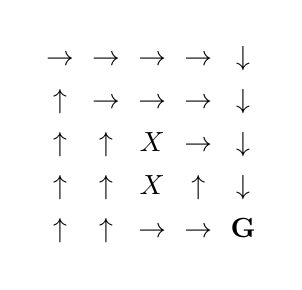
\begin{tikzpicture}
            \matrix (m) [matrix of nodes] {
                $\rightarrow$ & $\rightarrow$ & $\rightarrow$ & $\rightarrow$ & $\downarrow$ \\
                $\uparrow$ & $\rightarrow$ & $\rightarrow$ & $\rightarrow$ & $\downarrow$ \\
                $\uparrow$ & $\uparrow$ & $X$ & $\rightarrow$ & $\downarrow$ \\
                $\uparrow$ & $\uparrow$ & $X$ & $\uparrow$ & $\downarrow$ \\
                $\uparrow$ & $\uparrow$ & $\rightarrow$ & $\rightarrow$ & \textbf{G} \\
            };
        \end{tikzpicture}
        \caption{Policy by MCTS for 687-Grid World}
        \label{fig:arrow_grid_mcts}
    \end{minipage}
\end{figure}

\begin{figure}[H]
    \centering
    \begin{minipage}{0.48\textwidth}
        \centering
        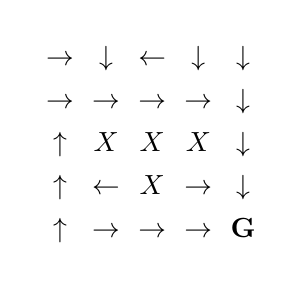
\begin{tikzpicture}
            \matrix (m) [matrix of nodes] {
                $\rightarrow$ & $\downarrow$ & $\leftarrow$ & $\downarrow$ & $\downarrow$ \\
                $\rightarrow$ & $\rightarrow$ & $\rightarrow$ & $\rightarrow$ & $\downarrow$ \\
                $\uparrow$ & $X$ & $X$ & $X$ & $\downarrow$ \\
                $\uparrow$ & $\leftarrow$ & $X$ & $\rightarrow$ & $\downarrow$ \\
                $\uparrow$ & $\rightarrow$ & $\rightarrow$ & $\rightarrow$ & \textbf{G} \\
            };
        \end{tikzpicture}
        \caption{Policy by Value Iteration for Cat vs Monsters}
        \label{fig:arrow_cvm_value_iteration_mcts}
    \end{minipage}
    \hfill
    \begin{minipage}{0.48\textwidth}
        \centering
        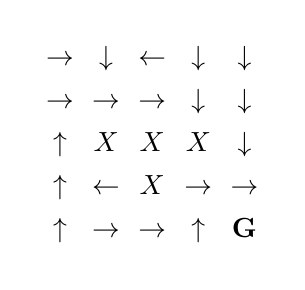
\begin{tikzpicture}
            \matrix (m) [matrix of nodes] {
                $\rightarrow$ & $\downarrow$ & $\leftarrow$ & $\downarrow$ & $\downarrow$ \\
                $\rightarrow$ & $\rightarrow$ & $\rightarrow$ & $\downarrow$ & $\downarrow$ \\
                $\uparrow$ & $X$ & $X$ & $X$ & $\downarrow$ \\
                $\uparrow$ & $\leftarrow$ & $X$ & $\rightarrow$ & $\rightarrow$ \\
                $\uparrow$ & $\rightarrow$ & $\rightarrow$ & $\uparrow$ & \textbf{G} \\
            };
        \end{tikzpicture}
        \caption{Policy by MCTS for Cat vs Monsters}
        \label{fig:arrow_cvm_mcts}
    \end{minipage}
\end{figure}

\begin{figure}[H]
    \centering
    \begin{minipage}{0.4\textwidth}
        \centering
        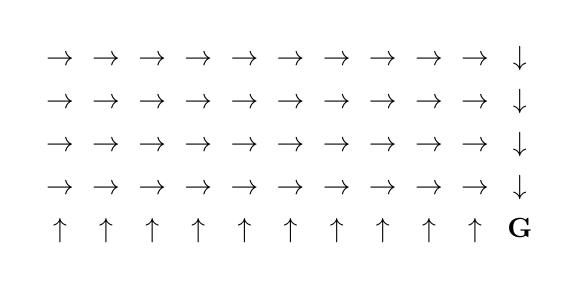
\begin{tikzpicture}
            \matrix (m) [matrix of nodes] {
                $\rightarrow$ & $\rightarrow$ & $\rightarrow$ & $\rightarrow$ & $\rightarrow$ & $\rightarrow$ & $\rightarrow$ & $\rightarrow$ & $\rightarrow$ & $\rightarrow$ & $\downarrow$ \\
                $\rightarrow$ & $\rightarrow$ & $\rightarrow$ & $\rightarrow$ & $\rightarrow$ & $\rightarrow$ & $\rightarrow$ & $\rightarrow$ & $\rightarrow$ & $\rightarrow$ & $\downarrow$ \\
                $\rightarrow$ & $\rightarrow$ & $\rightarrow$ & $\rightarrow$ & $\rightarrow$ & $\rightarrow$ & $\rightarrow$ & $\rightarrow$ & $\rightarrow$ & $\rightarrow$ & $\downarrow$ \\
                $\rightarrow$ & $\rightarrow$ & $\rightarrow$ & $\rightarrow$ & $\rightarrow$ & $\rightarrow$ & $\rightarrow$ & $\rightarrow$ & $\rightarrow$ & $\rightarrow$ & $\downarrow$ \\
                $\uparrow$ & $\uparrow$ & $\uparrow$ & $\uparrow$ & $\uparrow$ & $\uparrow$ & $\uparrow$ & $\uparrow$ & $\uparrow$ & $\uparrow$ & \textbf{G} \\
            };
        \end{tikzpicture}
        \caption{Policy by Value Iteration for Cliff Walking}
        \label{fig:arrow_cw_value_iteration_mcts}
    \end{minipage}
    \hfill
    \begin{minipage}{0.4\textwidth}
        \centering
        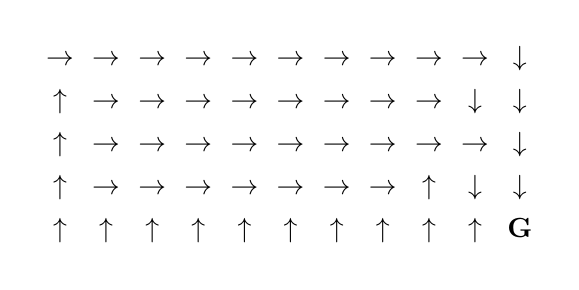
\begin{tikzpicture}
            \matrix (m) [matrix of nodes] {
                $\rightarrow$ & $\rightarrow$ & $\rightarrow$ & $\rightarrow$ & $\rightarrow$ & $\rightarrow$ & $\rightarrow$ & $\rightarrow$ & $\rightarrow$ & $\rightarrow$ & $\downarrow$ \\
                $\uparrow$ & $\rightarrow$ & $\rightarrow$ & $\rightarrow$ & $\rightarrow$ & $\rightarrow$ & $\rightarrow$ & $\rightarrow$ & $\rightarrow$ & $\downarrow$ & $\downarrow$ \\
                $\uparrow$ & $\rightarrow$ & $\rightarrow$ & $\rightarrow$ & $\rightarrow$ & $\rightarrow$ & $\rightarrow$ & $\rightarrow$ & $\rightarrow$ & $\rightarrow$ & $\downarrow$ \\
                $\uparrow$ & $\rightarrow$ & $\rightarrow$ & $\rightarrow$ & $\rightarrow$ & $\rightarrow$ & $\rightarrow$ & $\rightarrow$ & $\uparrow$ & $\downarrow$ & $\downarrow$ \\
                $\uparrow$ & $\uparrow$ & $\uparrow$ & $\uparrow$ & $\uparrow$ & $\uparrow$ & $\uparrow$ & $\uparrow$ & $\uparrow$ & $\uparrow$ & \textbf{G} \\
            };
        \end{tikzpicture}
        \caption{Policy by MCTS for Cliff Walking}
        \label{fig:arrow_cw_mcts}
    \end{minipage}

    
\end{figure}
\textbf{Observations:}\\
We can see the left side policies are from value iteration with $\gamma=0.925$ for cat vs monsters from figure \ref{fig:arrow_cvm_value_iteration_mcts},$\gamma=0.9$ for cliff walking from figure \ref{fig:arrow_cw_value_iteration_mcts} and $\gamma=0.99$ for 687-grid world from figure \ref{fig:arrow_grid_value_iteration_mcts}.
The right side policies are from MCTS with $\gamma=0.925$ for cat vs monsters from figure \ref{fig:arrow_cvm_mcts},$\gamma=0.9$ for cliff walking from figure \ref{fig:arrow_cw_mcts} and $\gamma=0.99$ for 687-grid world from figure \ref{fig:arrow_grid_mcts}.\\

This is because the value iteration is a deterministic algorithm and it will always converge to the optimal policy. Whereas, MCTS is a stochastic algorithm and it will converge to the optimal policy only if it explores the entire state space. And more over greedy policy can be sometimes not optimal. Especially near the gaol state it happens as it can not explore more visits from neighbours. It wont use the depth mit as well as exploration constant to balance the exploration and exploitation. Also, there could be equal probable actions for those sates near goalstates.

\subsubsection{REINFORCE with baseline} 
\textbf{Preliminary Implementation}\\ 
For implementing REINFORCE with baseline, we used different neural network architectures and hyperparameters for different MDPs. It is because of the nature of the MDP and the closeness in the values to be estimated and more. 
For the MDP - Cat monster domain, implemented a neural network that is deepest of all which has 4 hidden layers and 128 nodes in each layer. Coupled these layers with non linearity activations such as ReLU for better learning. Choose a decaying learning rate that starts at 0.001 and decays for each 100 steps at a rate of 0.8. Choose these learning rates and architectures based on the time it takes to finish learning and the value it converges to. 
For the MDP - 687 Grid World, chose gamma as 0.95, chose relatively shallower networks for both, as compared to Cat Monster domain and fewer nodes. Since we dont have much rewards associated with each transition. This has a learning rate of 1e-3 but higher decay rate than the previous case because, it is less complex than the previous mdp so reaching the optimal value will be quicker than in cat monster case. Therefore reducing the learning rate and making this less complex works better. 
For the MDP - Cliff Walking, set high and complex network architecture because we have so many states to compare and optimize simultaneously, simultaneously didn't decay the learning rate much. Initialized it to 1e-3 and only decayed it by 0.99 for every 50 steps. Chose different architectures for both policy and value estimator models. Kept on tweaking the  parameters until it wasn't taking too long to learn and also gives good estimates. Also chose to end the episode if we exceed 1000 steps. This is because we have comparably more number of states, the agent might keep exploring or pick up one and be stuck into it. However this clipping is only required only at the beginning of the trainig process. As we move further into learning, it turns out to be redundant.
\begin{figure}[H]
    \centering
    \begin{minipage}{0.4\textwidth}
        \centering
        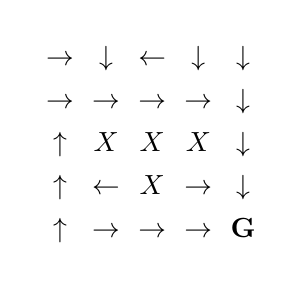
\begin{tikzpicture}
            \matrix (m) [matrix of nodes] {
                $\rightarrow$ & $\downarrow$ & $\leftarrow$ & $\downarrow$ & $\downarrow$ \\
                $\rightarrow$ & $\rightarrow$ & $\rightarrow$ & $\rightarrow$ & $\downarrow$ \\
                $\uparrow$ & $X$ & $X$ & $X$ & $\downarrow$ \\
                $\uparrow$ & $\leftarrow$ & $X$ & $\rightarrow$ & $\downarrow$ \\
                $\uparrow$ & $\rightarrow$ & $\rightarrow$ & $\rightarrow$ & \textbf{G} \\
            };
        \end{tikzpicture}
        \caption{Policy by Value Iteration for Cat Monster}
        \label{fig:arrow_grid_value_iteration}
    \end{minipage}
    \hfill
    \begin{minipage}{0.48\textwidth}
        \centering
        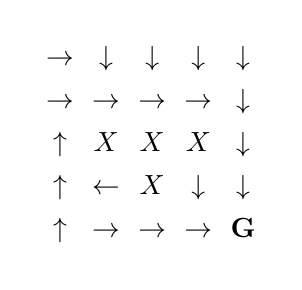
\begin{tikzpicture}
            \matrix (m) [matrix of nodes] {
                $\rightarrow$ & $\downarrow$ & $\downarrow$ & $\downarrow$ & $\downarrow$ \\
                $\rightarrow$ & $\rightarrow$ & $\rightarrow$ & $\rightarrow$ & $\downarrow$ \\
                $\uparrow$ & $X$ & $X$ & $X$ & $\downarrow$ \\
                $\uparrow$ & $\leftarrow$ & $X$ & $\downarrow$ & $\downarrow$ \\
                $\uparrow$ & $\rightarrow$ & $\rightarrow$ & $\rightarrow$ & \textbf{G} \\
            };
        \end{tikzpicture}
        \caption{Greedy Policy by REINFORCE with baseline for Cat monster MDP}
        \label{fig:arrow_grid_mcts}
    \end{minipage}
\end{figure}

\begin{figure}[H]
    \centering
    \begin{minipage}{0.48\textwidth}
        \centering
        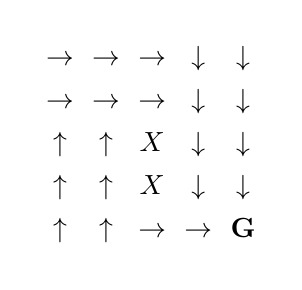
\begin{tikzpicture}
            \matrix (m) [matrix of nodes] {
                $\rightarrow$ & $\rightarrow$ & $\rightarrow$ & $\downarrow$ & $\downarrow$ \\
                $\rightarrow$ & $\rightarrow$ & $\rightarrow$ & $\downarrow$ & $\downarrow$ \\
                $\uparrow$ & $\uparrow$ & $X$ & $\downarrow$ & $\downarrow$ \\
                $\uparrow$ & $\uparrow$ & $X$ & $\downarrow$ & $\downarrow$ \\
                $\uparrow$ & $\uparrow$ & $\rightarrow$ & $\rightarrow$ & \textbf{G} \\
            };
        \end{tikzpicture}
        \caption{Policy by Value Iteration for 687-Grid World}
        \label{fig:arrow_grid_value_iteration}
    \end{minipage}
    \hfill
    \begin{minipage}{0.48\textwidth}
        \centering
        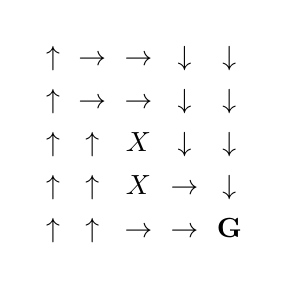
\begin{tikzpicture}
            \matrix (m) [matrix of nodes] {
                $\uparrow$ & $\rightarrow$ & $\rightarrow$ & $\downarrow$ & $\downarrow$ \\
                $\uparrow$ & $\rightarrow$ & $\rightarrow$ & $\downarrow$ & $\downarrow$ \\
                $\uparrow$ & $\uparrow$ & $X$ & $\downarrow$ & $\downarrow$ \\
                $\uparrow$ & $\uparrow$ & $X$ & $\rightarrow$ & $\downarrow$ \\
                $\uparrow$ & $\uparrow$ & $\rightarrow$ & $\rightarrow$ & \textbf{G} \\
            };
        \end{tikzpicture}
        \caption{Greedy Policy by REINFORCE with baseline for 687-Grid World}
        \label{fig:arrow_grid_mcts}
    \end{minipage}
\end{figure}

\begin{figure}[H]
    \centering
    \begin{minipage}{0.4\textwidth}
        \centering
        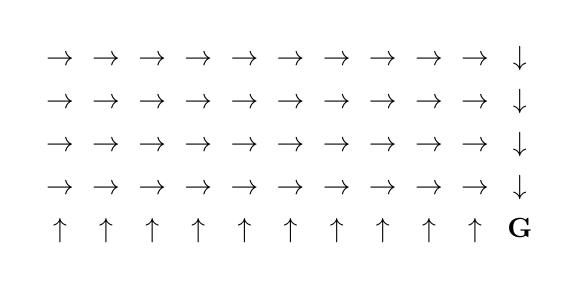
\begin{tikzpicture}
            \matrix (m) [matrix of nodes] {
                $\rightarrow$ & $\rightarrow$ & $\rightarrow$ & $\rightarrow$ & $\rightarrow$ & $\rightarrow$ & $\rightarrow$ & $\rightarrow$ & $\rightarrow$ & $\rightarrow$ & $\downarrow$ \\
                $\rightarrow$ & $\rightarrow$ & $\rightarrow$ & $\rightarrow$ & $\rightarrow$ & $\rightarrow$ & $\rightarrow$ & $\rightarrow$ & $\rightarrow$ & $\rightarrow$ & $\downarrow$ \\
                $\rightarrow$ & $\rightarrow$ & $\rightarrow$ & $\rightarrow$ & $\rightarrow$ & $\rightarrow$ & $\rightarrow$ & $\rightarrow$ & $\rightarrow$ & $\rightarrow$ & $\downarrow$ \\
                $\rightarrow$ & $\rightarrow$ & $\rightarrow$ & $\rightarrow$ & $\rightarrow$ & $\rightarrow$ & $\rightarrow$ & $\rightarrow$ & $\rightarrow$ & $\rightarrow$ & $\downarrow$ \\
                $\uparrow$ & $\uparrow$ & $\uparrow$ & $\uparrow$ & $\uparrow$ & $\uparrow$ & $\uparrow$ & $\uparrow$ & $\uparrow$ & $\uparrow$ & \textbf{G} \\
            };
        \end{tikzpicture}
        \caption{Policy by Value Iteration for Cliff Walking}
        \label{fig:arrow_cw_value_iteration_mcts}
    \end{minipage}
    \hfill
    \begin{minipage}{0.4\textwidth}
        \centering
        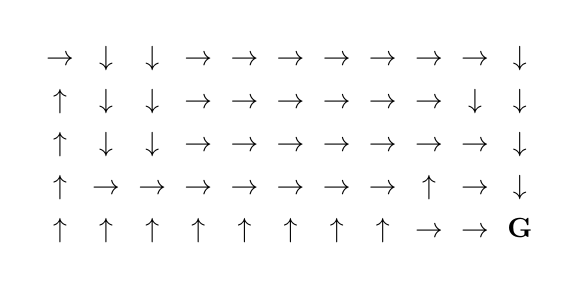
\begin{tikzpicture}
            \matrix (m) [matrix of nodes] {
                $\rightarrow$ & $\downarrow$ & $\downarrow$ & $\rightarrow$ & $\rightarrow$ & $\rightarrow$ & $\rightarrow$ & $\rightarrow$ & $\rightarrow$ & $\rightarrow$ & $\downarrow$ \\
                $\uparrow$ & $\downarrow$ & $\downarrow$ & $\rightarrow$ & $\rightarrow$ & $\rightarrow$ & $\rightarrow$ & $\rightarrow$ & $\rightarrow$ & $\downarrow$ & $\downarrow$ \\
                $\uparrow$ & $\downarrow$ & $\downarrow$ & $\rightarrow$ & $\rightarrow$ & $\rightarrow$ & $\rightarrow$ & $\rightarrow$ & $\rightarrow$ & $\rightarrow$ & $\downarrow$ \\
                $\uparrow$ & $\rightarrow$ & $\rightarrow$ & $\rightarrow$ & $\rightarrow$ & $\rightarrow$ & $\rightarrow$ & $\rightarrow$ & $\uparrow$ & $\rightarrow$ & $\downarrow$ \\
                $\uparrow$ & $\uparrow$ & $\uparrow$ & $\uparrow$ & $\uparrow$ & $\uparrow$ & $\uparrow$ & $\uparrow$ & $\rightarrow$ & $\rightarrow$ & \textbf{G} \\
            };
        \end{tikzpicture}
        \caption{Policy by REINFORCE with baseline for Cliff Walking}
        \label{fig:arrow_cw_mcts}
    \end{minipage}
\end{figure}

\textbf{Observation:} We see that here that there is some variation to the policies learnt through value iteration and REINFORCE methods. One reason could be because of the stochastic nature of the policy that we have implemented. And it has approximately reached the convergence but not exactly. Also we choose actions based on the probability of each action being chosen not the best one. Hence we may have this slight error in the policies learnt.

\begin{figure}[h!]
    \centering
    \begin{subfigure}{0.3\textwidth}
        \includegraphics[width=\textwidth]{figs/reinforce_cm/pol_losses_running_mean.png}
        \caption{Policy loss for cat monster domain using REINFORCE with baseline}
        \label{fig:5}
    \end{subfigure}
    \begin{subfigure}{0.3\textwidth}
        \includegraphics[width=\textwidth]{figs/reinforce_cm/val_losses_running_mean.png}
        \caption{Value function loss for cat monster domain using REINFORCE with baseline}
        \label{fig:6}
    \end{subfigure}
    \begin{subfigure}{0.3\textwidth}
        \includegraphics[width=\textwidth]{figs/reinforce_cm/returns.png}
        \caption{Returns for cat monster domain using REINFORCE with baseline}
        \label{fig:7}
    \end{subfigure}
    \caption{Results for the cat monster domain using REINFORCE with baseline.}
    \label{fig:combined}
\end{figure}


\begin{figure}[h!]
    \centering
    \begin{subfigure}{0.3\textwidth}
        \includegraphics[width=\textwidth]{figs/reinforce_gw/val_losses_running_mean.png}
        \caption{Value loss for 687 grid world domain using REINFORCE with baseline}
        \label{fig:9}
    \end{subfigure}
    \begin{subfigure}{0.3\textwidth}
        \includegraphics[width=\textwidth]{figs/reinforce_gw/pol_losses_running_mean.png}
        \caption{Policy loss for 687 grid world domain using REINFORCE with baseline}
        \label{fig:8}
    \end{subfigure}
    \begin{subfigure}{0.3\textwidth}
        \includegraphics[width=\textwidth]{figs/reinforce_gw/eps_running_mean.png}
        \caption{Episodic returns for 687 grid world domain using REINFORCE with baseline}
        \label{fig:7}
    \end{subfigure}
    \caption{Results for the 687 grid world domain using REINFORCE with baseline.}
    \label{fig:gw_combined}
\end{figure}

\newpage
\textbf{Observation:} We see that here that the loss functions for both the algorithms for their policy and value estimators is decreasing and convering to almost 0. The complexity of the Cat Monster domain leads to higher variability and slower convergence compared to the Grid World domain. REINFORCE with a baseline successfully optimizes both policy and value networks, as evidenced by the decreasing losses and improving rewards in both domains.Simpler environments like Grid World are more suited for rapid convergence, while more complex environments like Cat Monster require robust training and hyperparameter tuning to achieve comparable results.
\begin{figure}[h!]
    \centering
    \begin{subfigure}{0.3\textwidth}
        \includegraphics[width=\textwidth]{figs/reinforce_cw/val_losses_running_mean.png}
        \caption{Value loss for 687 grid world domain using REINFORCE with baseline}
        \label{fig:9}
    \end{subfigure}
    \begin{subfigure}{0.3\textwidth}
        \includegraphics[width=\textwidth]{figs/reinforce_cw/pol_losses_running_mean.png}
        \caption{Policy loss for 687 grid world domain using REINFORCE with baseline}
        \label{fig:8}
    \end{subfigure}
    \begin{subfigure}{0.3\textwidth}
        \includegraphics[width=\textwidth]{figs/reinforce_cw/eps_running_mean.png}
        \caption{Episodic returns for 687 grid world domain using REINFORCE with baseline}
        \label{fig:7}
    \end{subfigure}
    \caption{Results for the 687 grid world domain using REINFORCE with baseline.}
    \label{fig:gw_combined}
\end{figure}
\textbf{Observation:} We see that initally only we need some step clipping because initial policies are poor. Hence the agent keeps exploring initially. So we need to clip them. After a certain state, we can see that the agent is learning and the losses are decreasing and even the estimates are also getting optimised as we move towards convergence.

\subsubsection{Actor Critic}
\textbf{Implementation Details}
Chose neural network based architecture and implemented these on cat monster and grid world domains. For every step, updated the weight parameters of both these architectures. It took a lot of time to implement comparable number of episodes for this method than REINFORCE with baseline. This is due to the concurrent training. The below plots were obtained which shows the 

\begin{figure}[h!]
    \centering
    \begin{subfigure}{0.3\textwidth}
        \includegraphics[width=\textwidth]{figs/arctic_cm/returns.png}
        \caption{Value loss for 687 grid world domain using REINFORCE with baseline}
        \label{fig:9}
    \end{subfigure}
    \begin{subfigure}{0.3\textwidth}
        \includegraphics[width=\textwidth]{figs/arctic_gw/returns.png}
        \caption{Episodic returns for 687 grid world domain using REINFORCE with baseline}
        \label{fig:7}
    \end{subfigure}
    \caption{Results for the 687 grid world domain using REINFORCE with baseline.}
    \label{fig:gw_combined}
\end{figure}

\textbf{Observation:}
The above plots were obtained after training actor critic agent. The plot still needs further finetuning but this is where it stands as of now.

\section{Tasks}
\begin{itemize}
    \item Avinash Nandyala - MCTS implementation, on all 4 domains, Actor critic implementation and report writing
    \item Sneha Sree Vavilapalli - MCTS implemetation 2 domains (687-Grid World, cats vs Monsters), REINFORCE with baseline implementation on all the 3 domains, Actor Critic implementation and report writing
\end{itemize}

\end{document}